%% 
%% Copyright 2019-2021 Elsevier Ltd
%% 
%% This file is part of the 'CAS Bundle'.
%% --------------------------------------
%% 
%% It may be distributed under the conditions of the LaTeX Project Public
%% License, either version 1.2 of this license or (at your option) any
%% later version.  The latest version of this license is in
%%    http://www.latex-project.org/lppl.txt
%% and version 1.2 or later is part of all distributions of LaTeX
%% version 1999/12/01 or later.
%% 
%% The list of all files belonging to the 'CAS Bundle' is
%% given in the file `manifest.txt'.
%% 
%% Template article for cas-dc documentclass for 
%% double column output.

\documentclass[a4paper,fleqn]{cas-dc}
\usepackage{cleveref}
\usepackage{placeins}
\usepackage{afterpage}


% If the frontmatter runs over more than one page
% use the longmktitle option.

%\documentclass[a4paper,fleqn,longmktitle]{cas-dc}

% \usepackage[numbers]{natbib}
\usepackage[authoryear]{natbib}
% \usepackage[authoryear,longnamesfirst]{natbib}

%%%Author macros
\def\tsc#1{\csdef{#1}{\textsc{\lowercase{#1}}\xspace}}
\tsc{WGM}
\tsc{QE}
%%%

% Uncomment and use as if needed
%\newtheorem{theorem}{Theorem}
%\newtheorem{lemma}[theorem]{Lemma}
%\newdefinition{rmk}{Remark}
%\newproof{pf}{Proof}
%\newproof{pot}{Proof of Theorem \ref{thm}}

\renewcommand{\dblfloatpagefraction}{0.4}

\begin{document}
\let\WriteBookmarks\relax
\def\floatpagepagefraction{1}
\def\textpagefraction{.001}

% Short title
% \shorttitle{<short title of the paper for running head>}    
\shorttitle{Weightage-based Supervised Learning System.}

% Short author
% \shortauthors{<short author list for running head>}  
\shortauthors{Ketkar Y., Gawade S.}

% Main title of the paper
\title [mode = title]{Detection of Arrhythmia Using Weightage-based Supervised Learning System for COVID-19.}

\let\printorcid\relax

% Title footnote mark
% eg: \tnotemark[1]
% \tnotemark[<tnote number>] 

% Title footnote 1.
% eg: \tnotetext[1]{Title footnote text}
% \tnotetext[<tnote number>]{<tnote text>} 

% First author
%
% Options: Use if required
% eg: \author[1,3]{Author Name}[type=editor,
%       style=chinese,
%       auid=000,
%       bioid=1,
%       prefix=Sir,
%       orcid=0000-0000-0000-0000,
%       facebook=<facebook id>,
%       twitter=<twitter id>,
%       linkedin=<linkedin id>,
%       gplus=<gplus id>]

\author[1]{Yashodhan Ketkar}

% Corresponding author indication
% \cormark[<corr mark no>]

% Footnote of the first author
% \fnmark[<footnote mark no>]

% Email id of the first author
\ead{ketkaryapr19me@student.mes.ac.in}

% URL of the first author
% \ead[url]{<URL>}

% Credit authorship
% eg: \credit{Conceptualization of this study, Methodology, Software}
% \credit{<Credit authorship details>}

% Address/affiliation
\affiliation[1]{organization={Department of Information Technology Engineering, Pillai College of Engineering},
            % addressline={}, 
            city={Panvel},
%          citysep={}, % Uncomment if no comma needed between city and postcode
            postcode={410206}, 
            state={Maharashtra},
            country={India}}

\author[2]{Sushopti Gawade}

% Footnote of the second author
% \fnmark[2]

% Email id of the second author
\ead{sgawade@mes.ac.in}

% URL of the second author
% \ead[url]{}

% Credit authorship
% \credit{}

% Address/affiliation
\affiliation[2]{organization={Department of Computer Engineering, Pillai College of Engineering},
            % addressline={}, 
            city={Panvel},
%          citysep={}, % Uncomment if no comma needed between city and postcode
            postcode={410206}, 
            state={Maharashtra},
            country={India}}

% Corresponding author text
% \cortext[2]{Corresponding author}

% Footnote text
% \fntext[1]{}

% For a title note without a number/mark
%\nonumnote{}

% Here goes the abstract
\begin{abstract}
COVID-19 disease became a global pandemic in the last few years. This disease was highly contagious, and it quickly spread throughout several countries. Its infection can lead to severe implications in its victims, including cardiovascular issues. This complication develops in some people with a history of cardiovascular illness, whereas it emerges in others after COVID-19 infection. Cardiovascular problems are the primary cause of mortality in COVID-19 patients and are used to predict disease prognosis. Identifying arrhythmia from abnormalities in patient ECG signals is one approach to the detection of cardiovascular disorders. This is a laborious and time-consuming procedure that can be automated. The proposed method selects the most suitable model for this task. The selection is done through the weightage generated from the user's requirements. The proposed method uses supervised learning to identify abnormalities in ECG waves. The models provided by the selection system during tests were able to meet user requirements. The models achieved up to 97\% accuracy and 97\% precision in predictive tasks.
\end{abstract}

% Use if graphical abstract is present
%\begin{graphicalabstract}
%\includegraphics{}
%\end{graphicalabstract}

% Research highlights
% \begin{highlights}
% \item a
% \item a
% \item a
% \end{highlights}

% Keywords
% Each keyword is seperated by \sep
\begin{keywords}
    Arrhythmia Detection \sep
    Automated Model Generation \sep
    Automated Model Training \sep
    Machine Learnign In Healthcare \sep
    Supervised Learning Algoirthm \sep
    Weightage based Model Selection \sep
\end{keywords}

\tolerance 9999
\maketitle


% Main text
% \section{Introduction}\label{sec:introduction}
\section{Introduction} \label{sec:introduction}

COVID-19 has been widespread in recent years. It targets the human respiratory system, causing severe respiratory issues. Depending on a person's condition and the prevalence of comorbidities, this disease can be fatal. Cardiovascular comorbidities are frequent in COVID-19 disease. Cardiovascular comorbidities are also problematic to diagnose in the absence of suitable equipment. Checking for arrhythmia in patients is one approach to detection. Arrhythmia is the irregular beating of the heart. Arrhythmia is detected by examining ECG signals. Because COVID-19 has put a strain on the medical personnel, detection takes longer than usual. Increased Internet connectivity has led to the use of machine learning and artificial intelligence (AI) for service in a variety of sectors. This increases research in the field of machine learning and has an impact on machine learning in a variety of domains. One of them is the medical and healthcare businesses. Machine learning is used to detect and categorize viruses and other microorganisms in patients. In medical applications, machine learning algorithms have already been shown to be quite useful.

The machine learning system may be used to scan these ECG signals and detect them. These signs may be detected considerably faster and more efficiently using supervised learning techniques. In such exact classification problems, supervised algorithms have previously been demonstrated to be quicker than unsupervised techniques. Once taught, this algorithm may also be utilized to make future predictions.

There are several supervised algorithms accessible, allowing us to select the best method for our purposes. This phase can be automated in the case of the general population. A few methods may be pre-programmed into the system, and the computer can then train and pick the best model for the supplied dataset. This will free up medical personnel to focus on patient care and problem-solving.

\section{Literature Review} \label{sec:literature_review}

\cite*{02_rp} suggest that arrhythmia is one of the most common symptoms in patients with COVID19. {\responsemod Arrhythmia was found in 7\% of all Wuhan COVID-19 cases and 14.8\% of patients with poor outcomes.} \cite*{18_rp} state that 17\% of patients hospitalized in China were diagnosed with arrhythmia. \citeauthor{18_rp} conducted a review of 10 eligible studies (5,193 patients) for analysis and found that atrial arrhythmia was present in 9.2\% of cases. A review by \cite*{15_rp} of 17 studies with 5,815 patients showed that arrhythmia was detected in 9.3\% of COVID-19 cases. \cite*{25_rp} suggest that only 8\% of patients with arrhythmia had prior cardiovascular conditions. {\responsemod \citeauthor{25_rp} also mentioned that 56\% of patients showed symptoms after the COVID-19 infection.}

\cite*{24_rp} used an ensemble classifier to detect the anomalies in the ECG signal. This approach, which combines multiple classifiers for prediction, has proven effective because the accuracy of the ensemble classifier is significantly higher than that of a single classifier. A few authors used this approach to improve the prediction accuracy of supervised learning models. \cite*{10_rp} used the maximal overlap wavelet packet transform ensemble with a neural network and achieved satisfactory results. \cite*{20_rp} used the ensemble approach to predict the results of the students. \citeauthor{20_rp} state the model was able to predict the correct results even with a small amount of training data. \cite*{16_rp} compared the FLINK-based iForest ensembled algorithms against the sklearn-iForset and other algorithms. \citeauthor{16_rp} concluded that the Flink-iForest algorithm showed better performance than off-the-shelf algorithms. \cite*{11_rp} used the AutoML algorithm and tools on data streams. \citeauthor{11_rp} concluded that the default classifiers can be used with AutoML tools for accurate prediction. With AutoML tools, prediction systems can be automated.

\cite*{ref_paper_m1} used machine learning for the prediction of end-of-semester results. \cite*{ref_paper_m1} used SVM, KNN, and DT models. \cite*{ref_paper_m1} concluded that the machine learning system performed satisfactorily, with SVM achieving up to 78\% accuracy.

\cite*{23_rp} extracted appropriate features for the detection of epileptic seizures. \citeauthor{23_rp} preprocessed data and used ML algorithms on the data. \citeauthor{23_rp} concluded that the supervised learning models showed more effectiveness than the unsupervised learning models. \cite*{12_rp} used a commercial classifier for the detection of arrhythmia. \citeauthor{12_rp} used ECG signals from patients and applied a custom SVM classifier. \citeauthor{12_rp} concluded that the algorithm was a successful and efficient {\responsemod detector} of arrhythmia.

\cite*{ref_paper_m2} used supervised learning algorithms for the early detection of heart disease and diabetes disease. \cite*{ref_paper_m2} concluded that the model performed satisfactorily.

\cite*{09_rp} used neural networks to process raw ECG signals and make predictions. {\responsemod While \cite*{22_rp} used small neural networks for efficient recognition processes, both studies concluded that artificial neural networks are extremely efficient and accurate in the prediction of anomalies.}

\cite*{06_rp} showed that the LDA classifier can outperform the SVM classifier in low-performance environments and lightweight systems. The self-learning algorithm makes the system more dynamic and adaptable to incoming signals. \cite*{14_rp} used adaptive fuzzy algorithms to classify ECG signals. \citeauthor{14_rp} stated that the algorithm showed satisfactory results, but it requires {\responsemod prior} classification patterns results. \cite*{ref_paper_self_rpa} suggest that the RPA system can be used in these systems for easier integration of machine learning with dynamic data. \cite*{21_rp} used ECG signals of COVID-19 patients for patient monitoring. \citeauthor{21_rp} used LSTM, SVM, and MLP algorithms to monitor data. \citeauthor{21_rp} suggest that machine learning with robotics can provide better results.

\cite*{07_rp} used a multi perceptron neural network for stroke predictions. The neural network showed high accuracy. \citeauthor{07_rp} were able to achieve up to 78\% accuracy. \citeauthor{07_rp} suggest that the model can produce better results with a larger training dataset. \cite*{05_rp} used artificial intelligence to detect heart disease. \citeauthor{05_rp} concluded that the algorithms achieved up to 83\% accuracy. \citeauthor{05_rp} also concluded that the system was able to comply with the HIPAA regulations.

\cite*{ref_paper_m3} used machine learning algorithms to predict crop growth rates. {\responsemod \citeauthor{ref_paper_m3} were able to get good insights into the field.} \citeauthor{ref_paper_m3} concluded that the use of machine learning will result in minimizing complexity and increasing yield in farming.

\cite*{01_rp} used a two-year dataset collected by Glumo Lake and used their expertise to train and select models. A mixed approach of data-driven and knowledge-driven modeling is used for the success of the application. \cite*{13_rp} used loo rate and stop criteria for model selection. \citeauthor{13_rp} investigated eight different issues and found that a larger loo rate was more desirable. \citeauthor{13_rp} also suggested that modeling difficulties can only be found by careful numerical calculations.

\cite*{17_rp} used a novel kernel to get the dataset description. \citeauthor{17_rp} concluded that this approach led to the discovery of invisible models. \citeauthor{17_rp} also state that this approach reduces the amount of human interaction. \cite*{04_rp} created a new model using the glmulti package. These models are unique and flexible. The model is automatically optimized to provide a multi-model interface. This approach allows you to quickly explore a large set of models for selection purposes. \cite*{08_rp} optimized parameters with a genetic algorithm. \citeauthor{08_rp} successfully used a genetic algorithm to reduce uncertainty in the prediction results. These methods can be used for the automated model selection system.

\section{Dataset and Method} \label{sec:dataset_and_method}

\subsection{Mathematical Model}\label{subsec:mathematical_model}

\Cref{fig:model_selection_approach} shows the approach toward the selection of a suitable model. With this system, we can handle up to N models. \Cref{eq:v_score} shows the mathematical formula used to calculate the V scores of the models. These V scores will allow the system to select the appropriate model.

\begin{equation}\label{eq:v_score}
    V_{score} = \left(\sum_{x=1}^{5} w_xP_x\right) - w_6^2P6
\end{equation}

\begin{figure*}
    \centering
    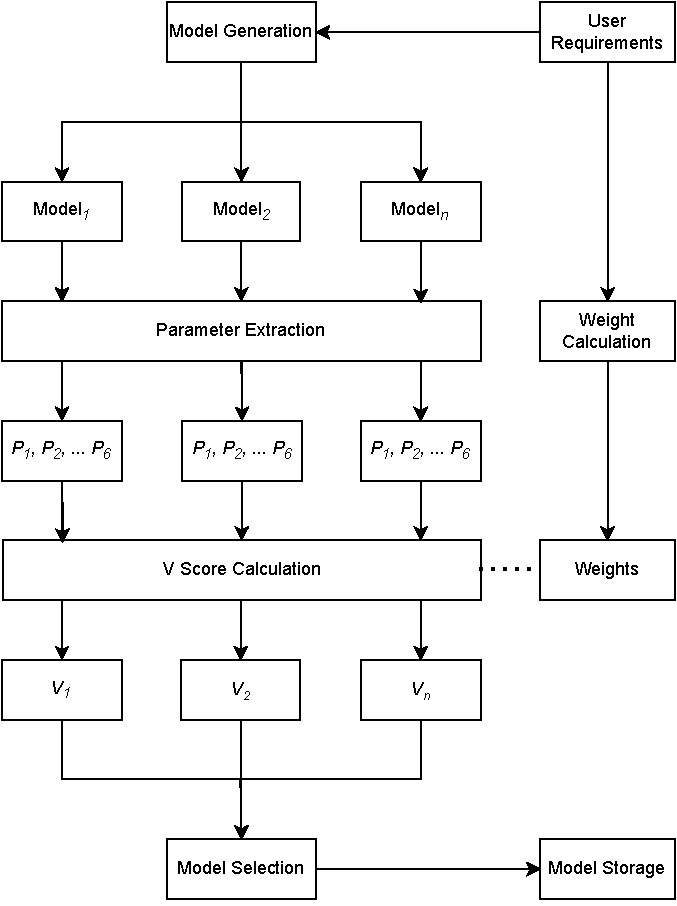
\includegraphics[width=1.2\columnwidth]{media/ch_dataset_and_methods/math_model_relaxed.pdf}
    \caption{Model Selection Approach}
    \label{fig:model_selection_approach}
\end{figure*}

\subsection{Method} \label{subsec:method}

\begin{figure*}[ht]
    \centering
    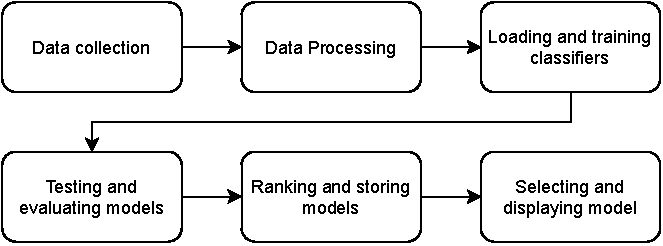
\includegraphics[width=1.2\columnwidth]{media/ch_dataset_and_methods/data_flow_system.pdf}
    \caption{Training and Selection Process}
    \label{fig:data_flow_in_system}
\end{figure*}

The \Cref{fig:data_flow_in_system}, shows the basic architecture of the automated model training and selection system. The data is collected from the user and processed by the application. This data is stored as training and testing datasets.

\begin{figure}[ht]
    \centering
    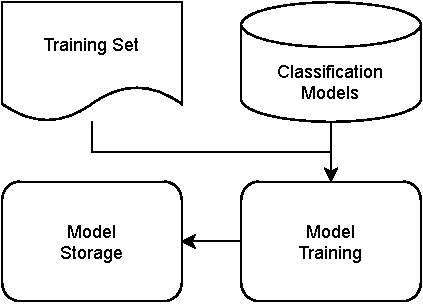
\includegraphics[width=0.7\columnwidth]{media/ch_dataset_and_methods/trainer.pdf}
    \caption{Training Process}
    \label{fig:training_process}
\end{figure}

\Cref{fig:training_process}, shows the training process. In this process, the training dataset is loaded into the system. Premade classification model templates are accessed by the system and trained with provided data. These trained models are stored by the system for the next step.

\begin{figure}[ht]
    \centering
    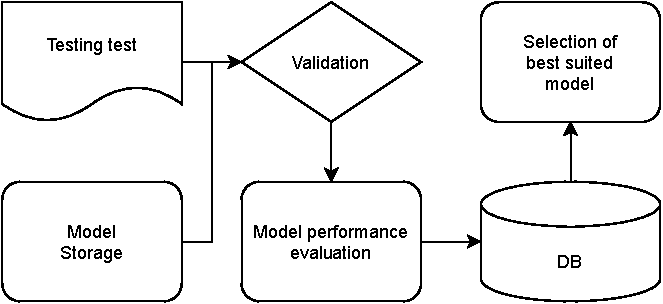
\includegraphics[width=0.7\columnwidth]{media/ch_dataset_and_methods/selector.pdf}
    \caption{Selection Process}
    \label{fig:selection_process}
\end{figure}

The \Cref{fig:selection_process}, shows the selection process. In this process, the testing dataset is used for the evaluation of the trained models. The trained models are ranked with respect to the performance evaluation. These ranks are used with the help of the tuning parameters to select the best-suited model. This model is stored as the best model for future classification.

\subsection{Dataset}
The ECG readings in this paper are obtained from the MIT-BIH arrhythmia database. This database is used for automated training and evaluation. This dataset was published in 1999 by MIT-BIH as an open-source database; it consists of training and testing datasets. This database is further divided into four equal parts for analysis. Each training set contains 21888 signals, and the testing set contains 5473 signals.
\section{Results And Testing} \label{sec:results_and_testing}
During the automated training and selection process, the SVM classifier is selected as the best-suited model for dataset 1, dataset 2, and dataset 4. Whereas RF classifier is selected as the best-suited model for dataset 3. 

Performance metrics used for evaluation were Accuracy, F1, Precision, Recall, Area under ROC Curve, and Total prediction time. The weightage assigned to these metrics for ranking was 1.0, 0.8, 0.4, 0.4, 0.4, 0.25 respectively. Where higher value means higher priority.

\subsection{Performance Evaluation} \label{subsec:performance_evaluation}
The models are tested with a testing dataset obtained from the MIT-BIH database. The testing dataset consists of 5473 signals. \Cref{fig:perfromance_results_dataset_1,fig:perfromance_results_dataset_2,fig:perfromance_results_dataset_3,fig:perfromance_results_dataset_4} shows that model trained with automated system produced satisfactory results. Few models like KNN, RF, and SVM performed better than other models (DT) at the cost of higher prediction time. Whereas MLP models produced good overall results with lower prediction time.
\Crefrange{tab:performance_of_models_trained_on_dataset_1}{tab:performance_of_models_trained_on_dataset_4} show the performance of the models on thier respcitve datasets in detail.

% Best model Performance chart
\begin{figure*}[ht]
    \centering
    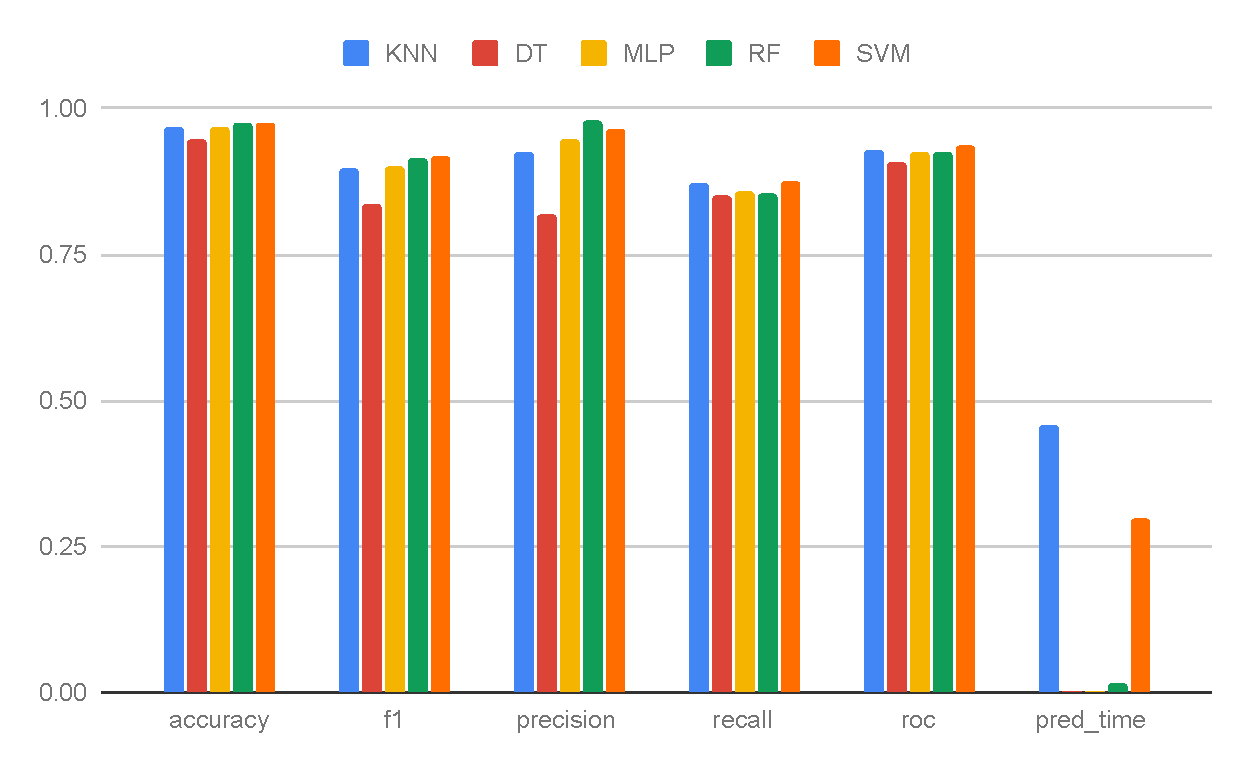
\includegraphics[width=1.9\columnwidth]{media/ch_result_and_testing/perf_ds_1.pdf}
    \caption{Performance Results Dataset 1} \label{fig:perfromance_results_dataset_1}
\end{figure*}

\begin{figure*}[ht]
    \centering
    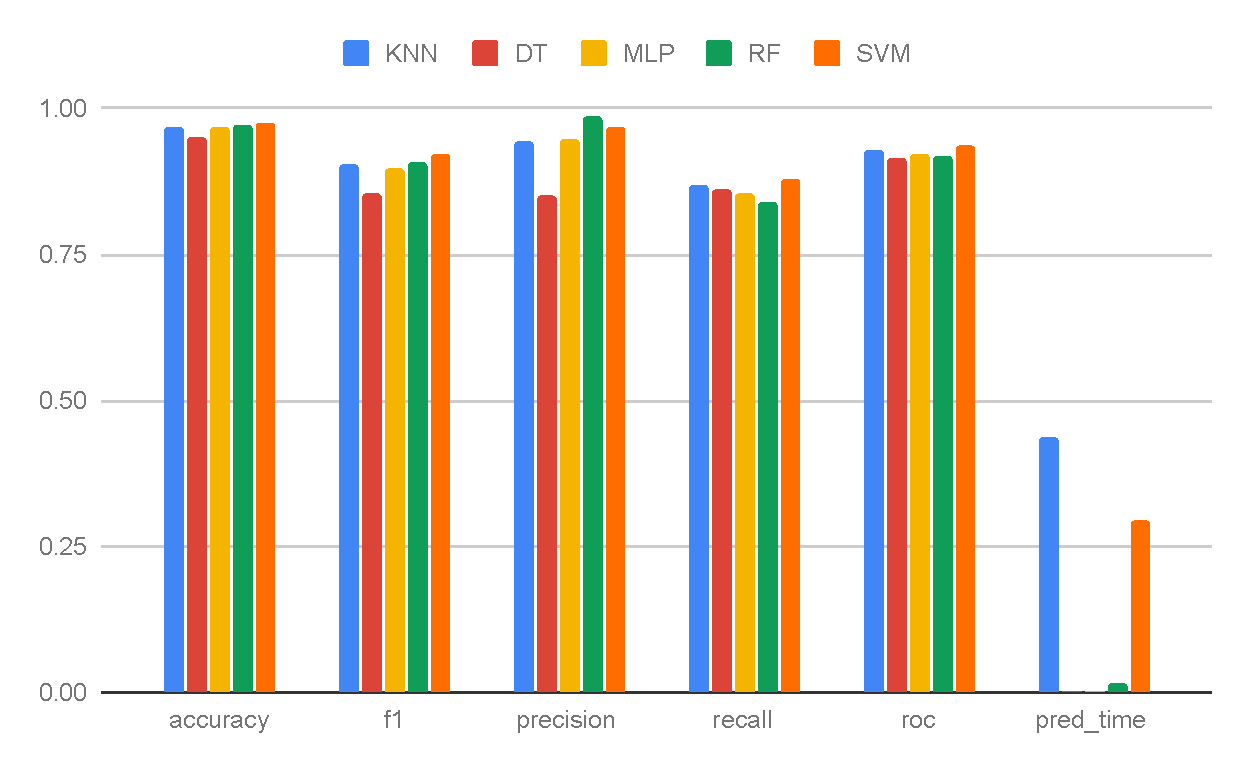
\includegraphics[width=1.9\columnwidth]{media/ch_result_and_testing/perf_ds_2.pdf}
    \caption{Performance Results Dataset 2} \label{fig:perfromance_results_dataset_2}
\end{figure*}

\begin{figure*}[ht]
    \centering
    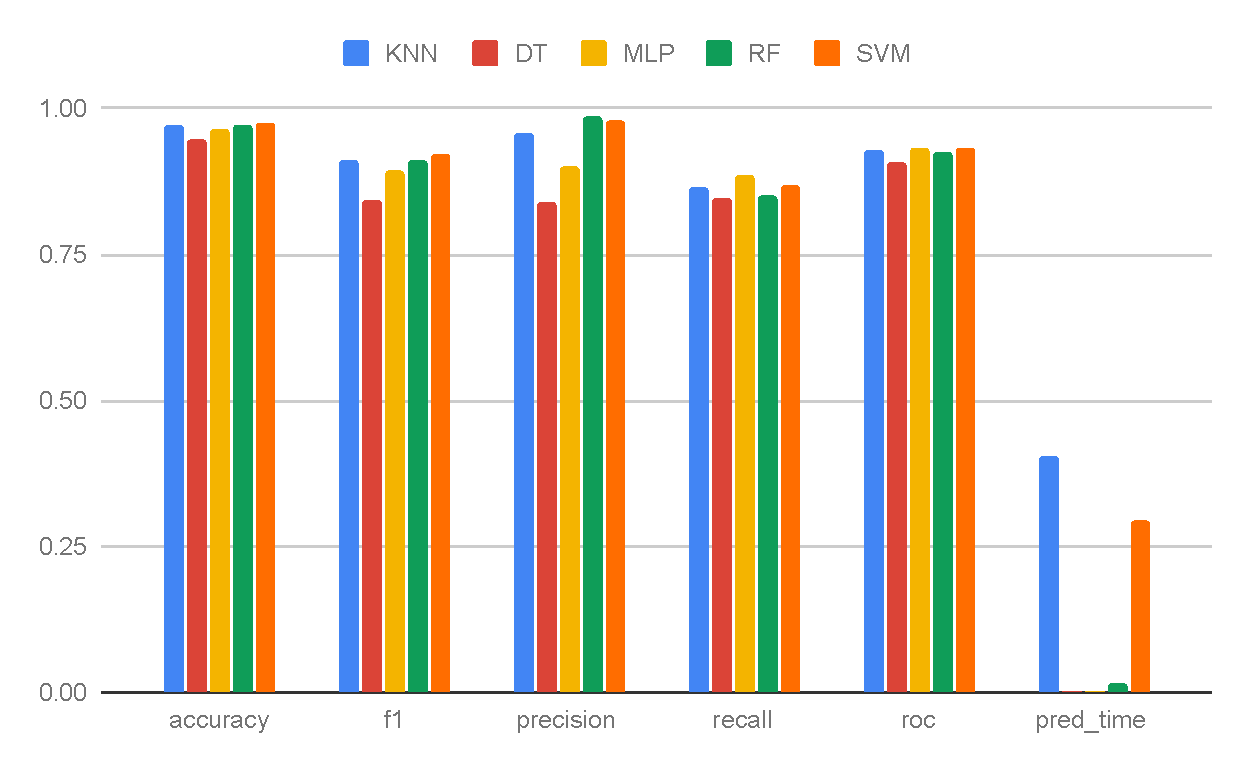
\includegraphics[width=1.9\columnwidth]{media/ch_result_and_testing/perf_ds_3.pdf}
    \caption{Performance Results Dataset 3} \label{fig:perfromance_results_dataset_3}
\end{figure*}

\begin{figure*}[ht]
    \centering
    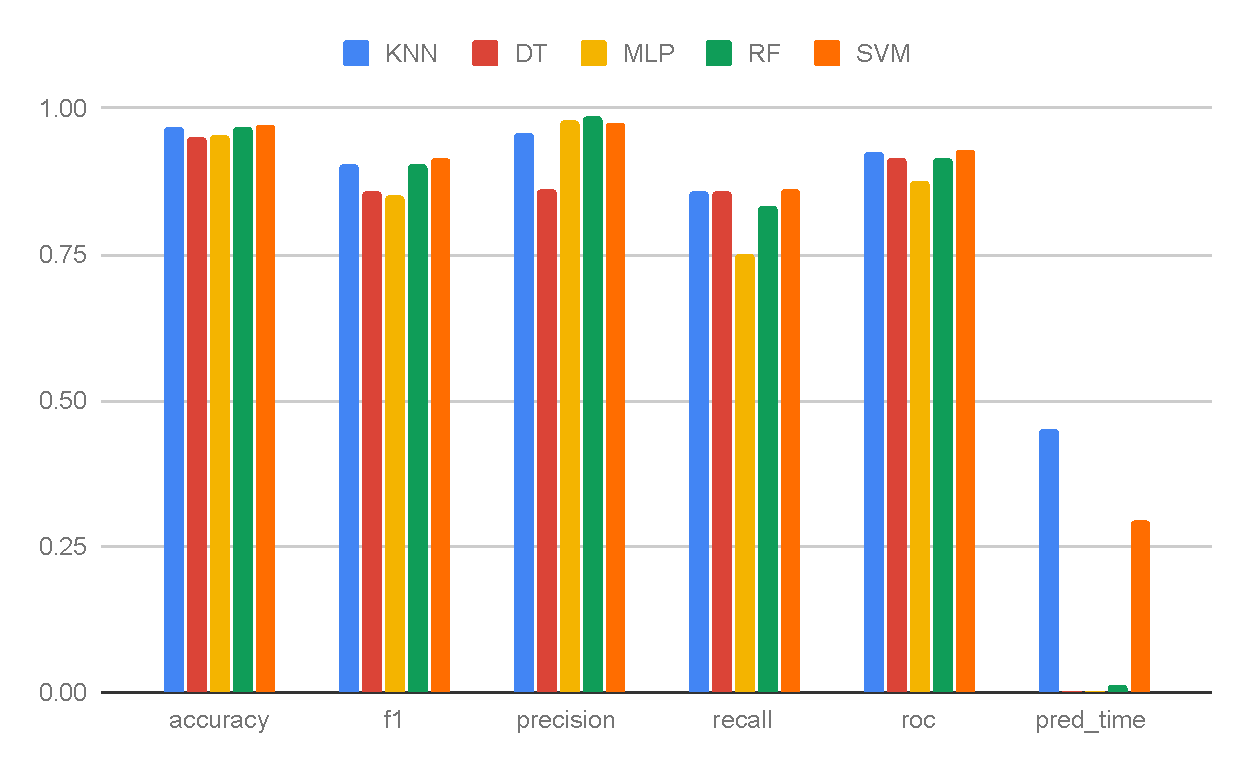
\includegraphics[width=1.9\columnwidth]{media/ch_result_and_testing/perf_ds_4.pdf}
    \caption{Performance Results Dataset 4} \label{fig:perfromance_results_dataset_4}
\end{figure*}

\subsection{Performance Error Calculation}
For error calculation, best models are tested against training datasets of other models. \Cref{fig:perfromance_delta_knn,fig:perfromance_delta_dt,fig:perfromance_delta_mlp,fig:perfromance_delta_rf,fig:perfromance_delta_svm} shows the average error introduced when models are tested against training datasets of other models. This chart shows that KNN, MLP, and SVM models introduced minimum errors, whereas DT and RF models introduced large amounts of error. \Cref{fig:perfromance_delta_svm} also shows that SVM model produced similar error across all datasets. This smaller difference in error suggests that the SVM classifier can be used for classification tasks of similar nature. \Crefrange{tab:performance_of_decision_tree_model_trained_on_dataset_1}{tab:performance_of_svm_model_trained_on_dataset_4} show the performance of the models when tested on other datasets in detail.

\begin{figure*}[ht]
    \centering
    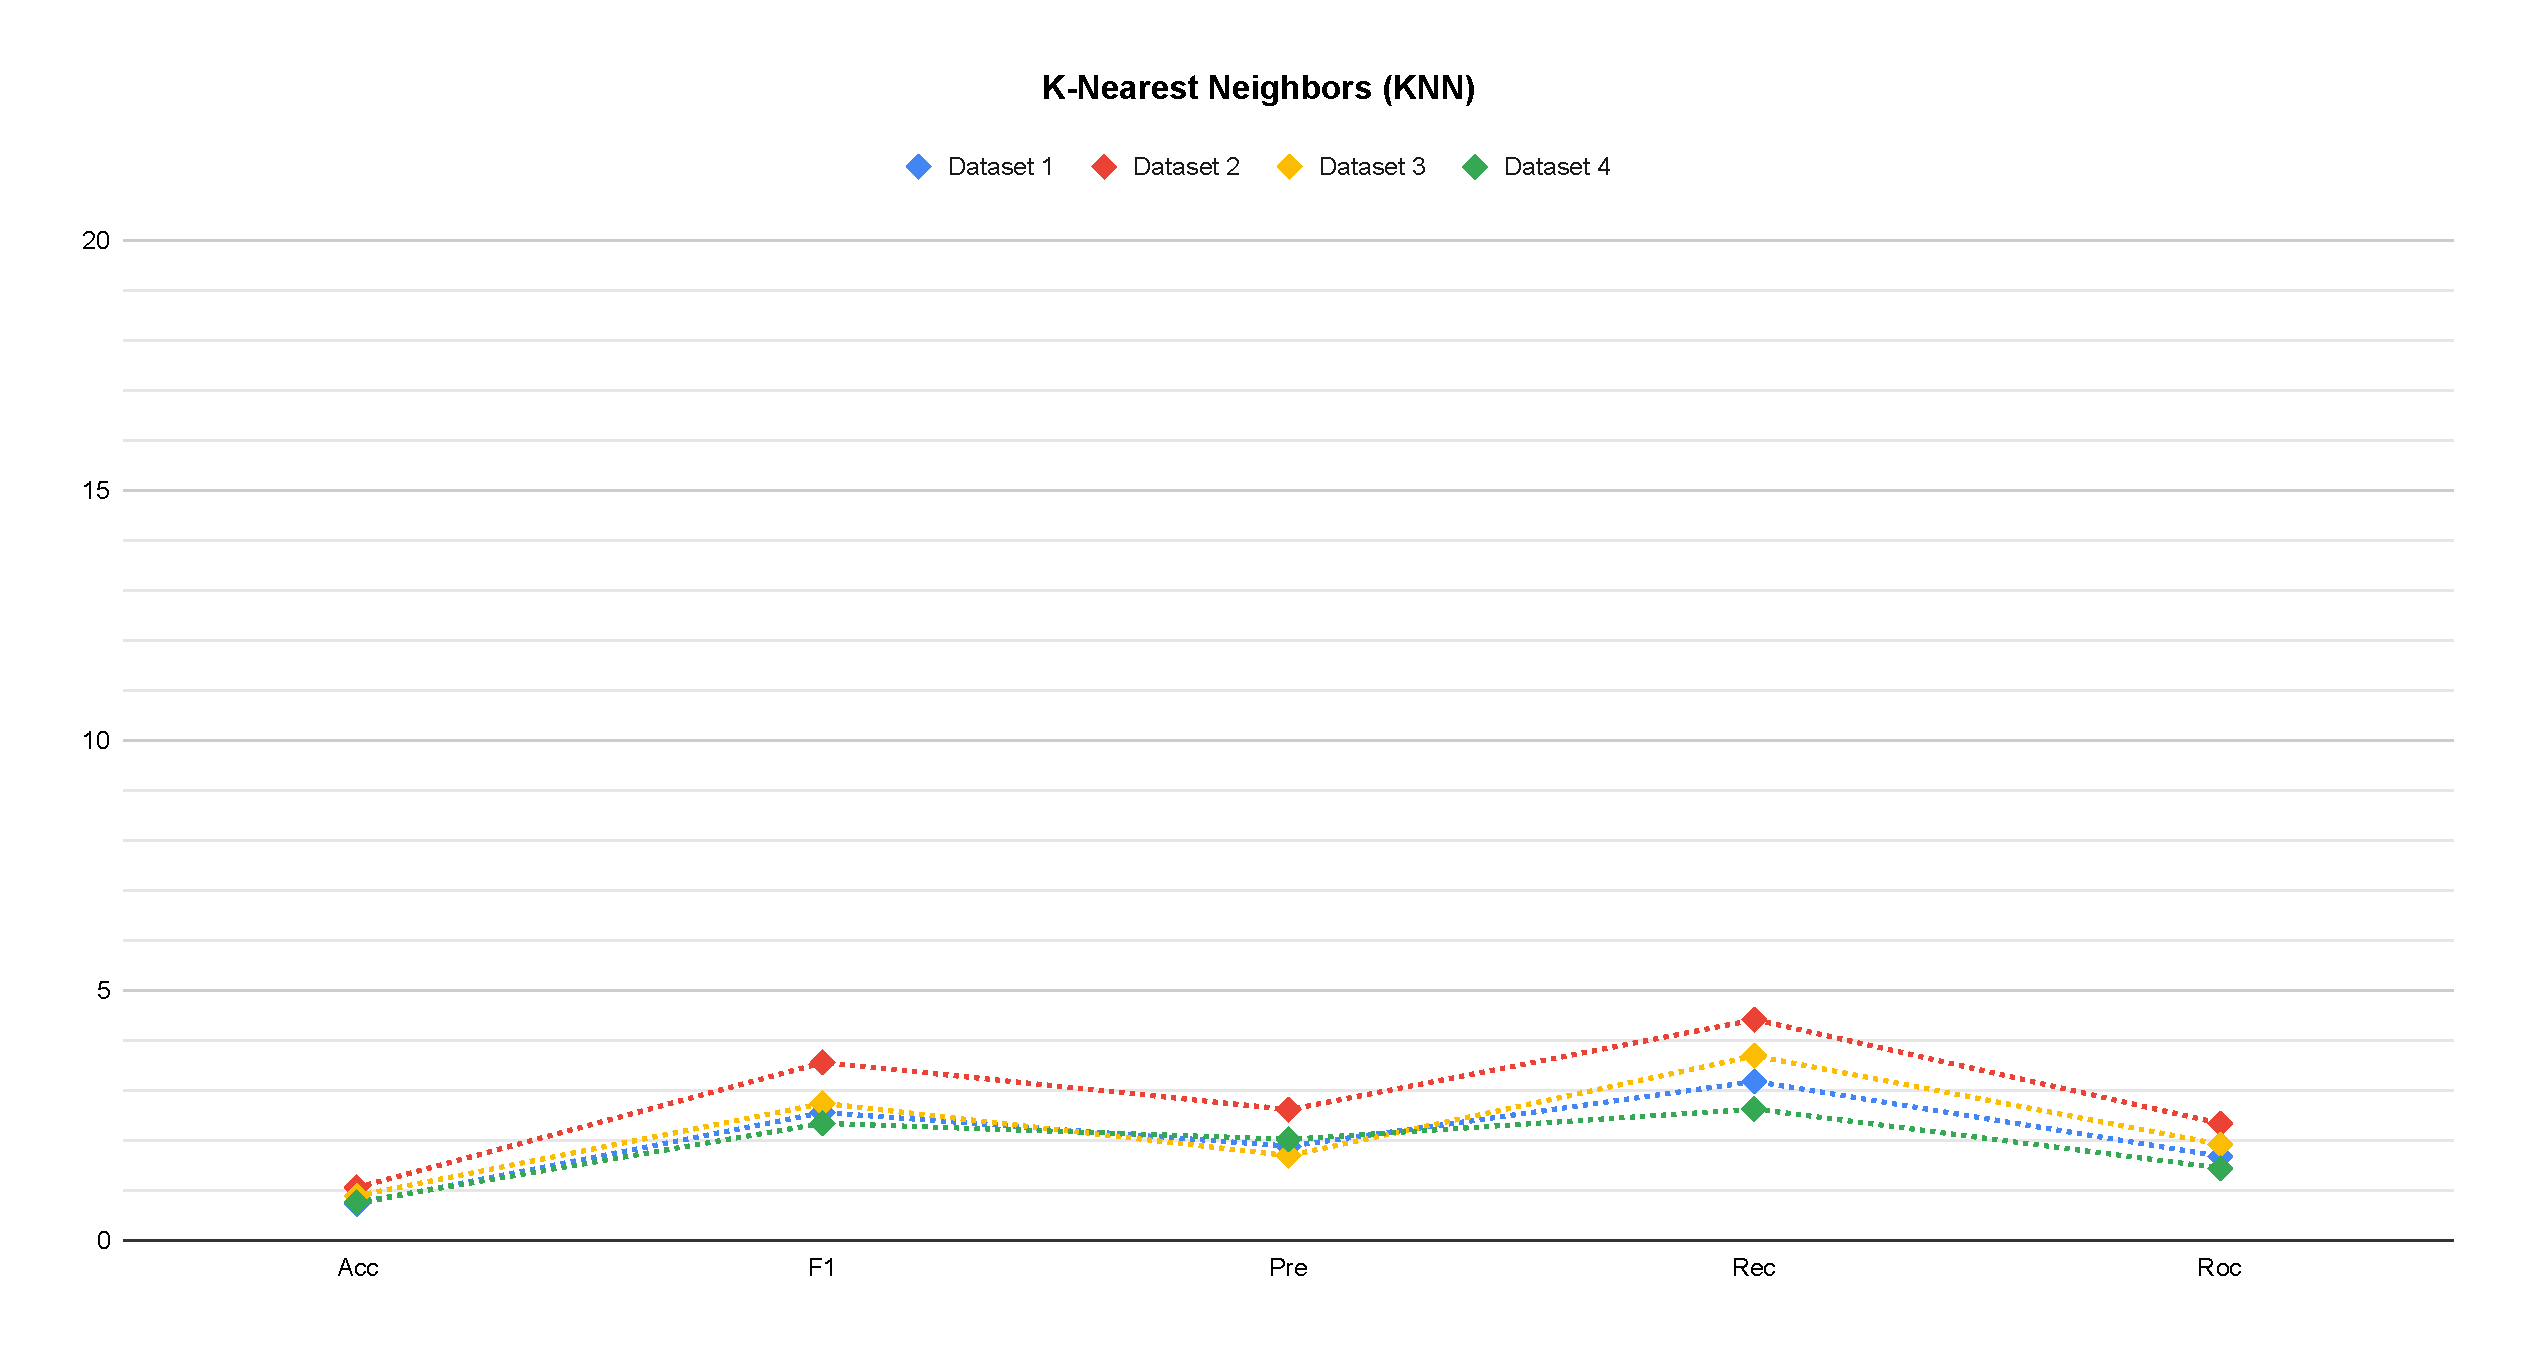
\includegraphics[width=1.9\columnwidth]{media/ch_result_and_testing/delta_KNN.pdf}
    \caption{Average Error for K-Nearest Neighbors (KNN) model} \label{fig:perfromance_delta_knn}
\end{figure*}

\begin{figure*}[ht]
    \centering
    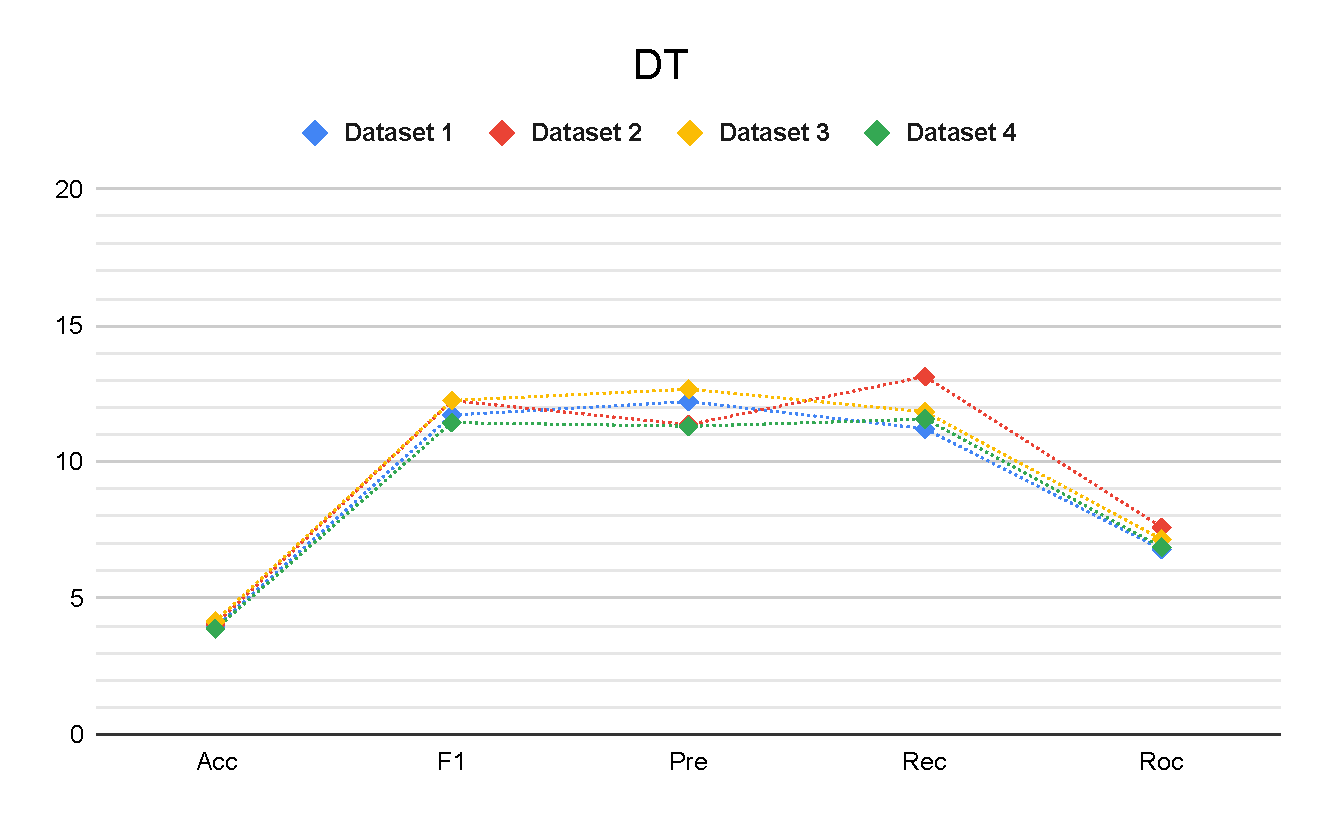
\includegraphics[width=1.9\columnwidth]{media/ch_result_and_testing/delta_DT.pdf}
    \caption{Average Error for Decision Tree (DT) model} \label{fig:perfromance_delta_dt}
\end{figure*}

\begin{figure*}[ht]
    \centering
    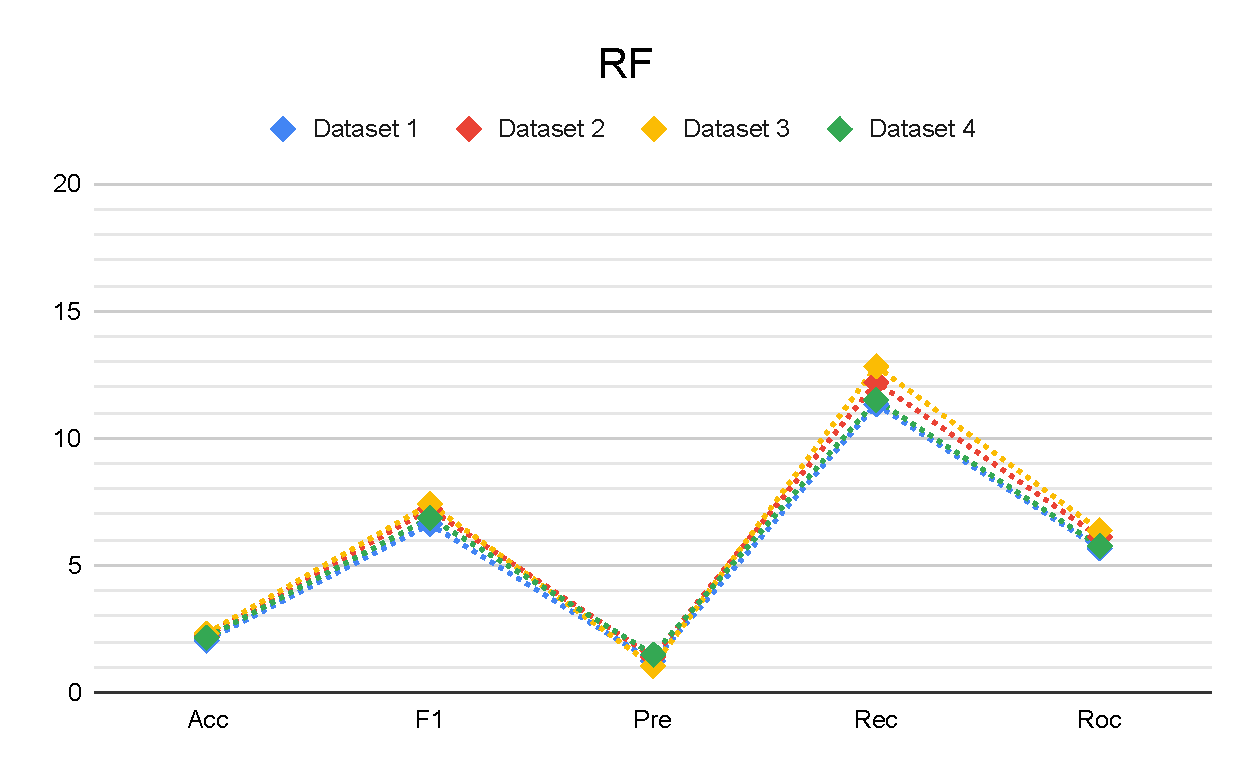
\includegraphics[width=1.9\columnwidth]{media/ch_result_and_testing/delta_RF.pdf}
    \caption{Average Error for Random Forest (RF) model} \label{fig:perfromance_delta_rf}
\end{figure*}

\begin{figure*}[ht]
    \centering
    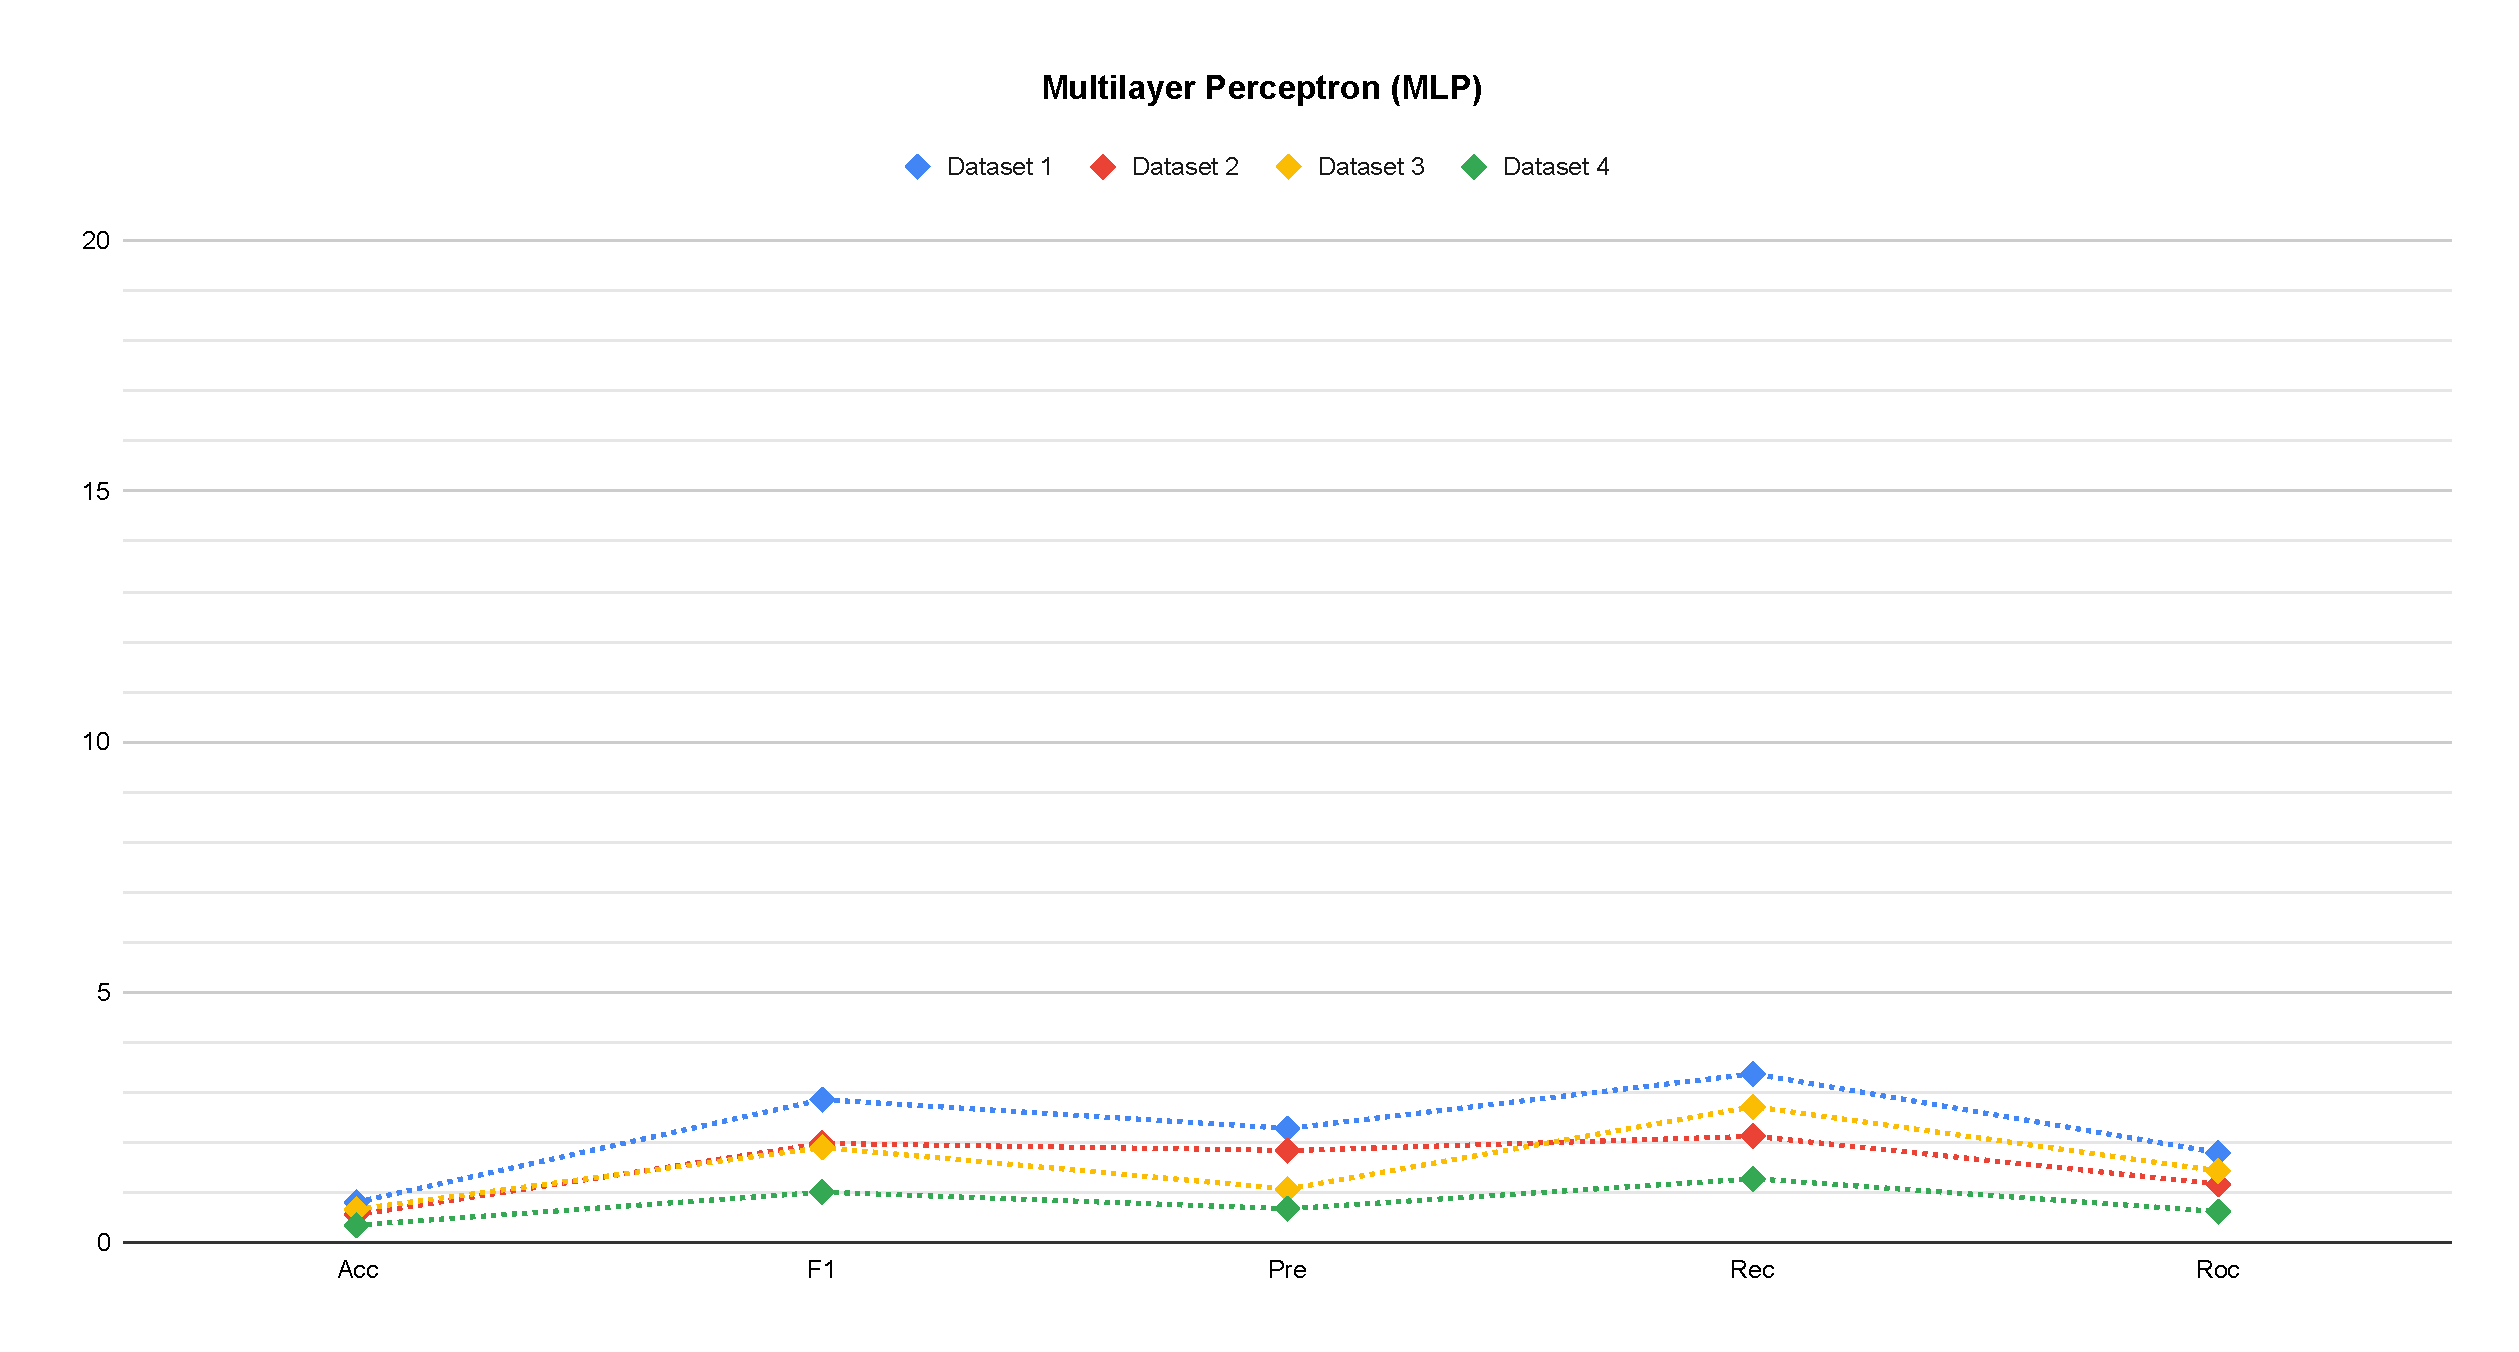
\includegraphics[width=1.9\columnwidth]{media/ch_result_and_testing/delta_MLP.pdf}
    \caption{Average Error for Multilayer Perceptron (MLP) model} \label{fig:perfromance_delta_mlp}
\end{figure*}

\begin{figure*}[ht]
    \centering
    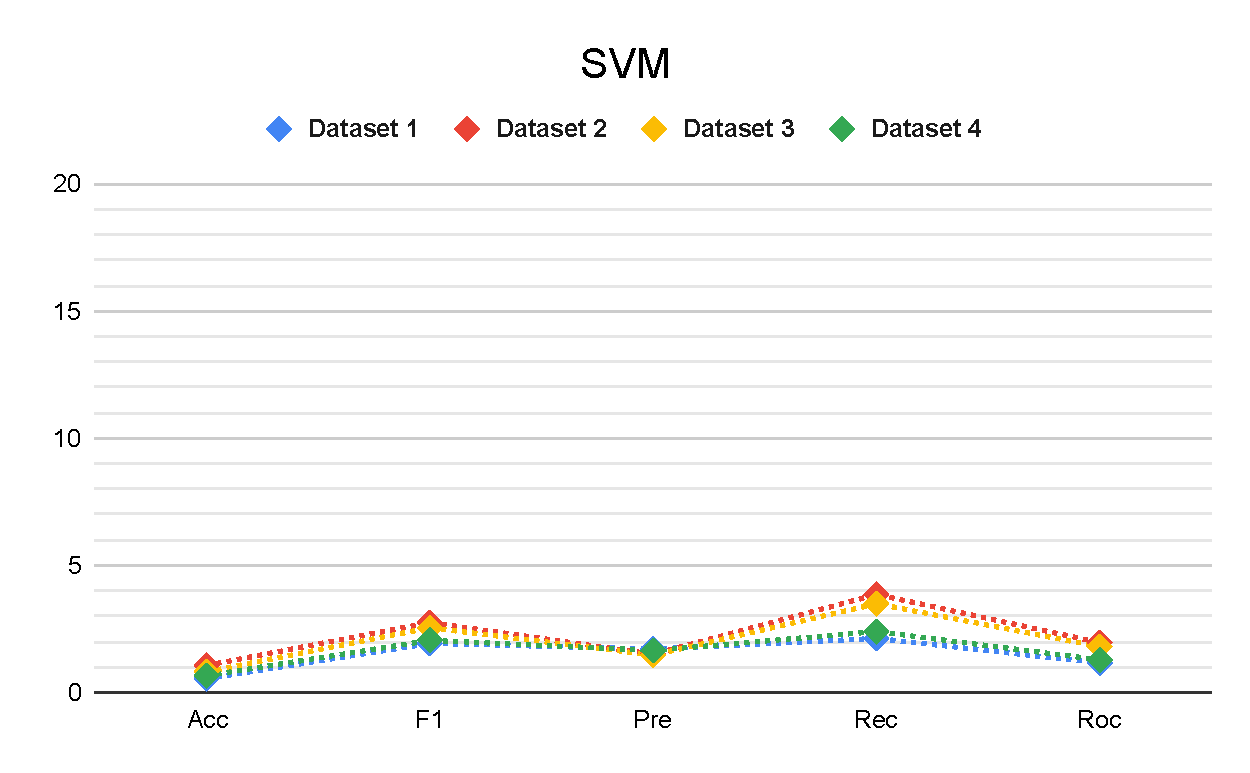
\includegraphics[width=1.9\columnwidth]{media/ch_result_and_testing/delta_SVM.pdf}
    \caption{Average Error for Support Vector Machine (SVM) model} \label{fig:perfromance_delta_svm}
\end{figure*}

\section{Conclusion and Future Work}\label{sec:conclusion_and_futur_work}

The system performed satisfactorily during the tests. The application was able to select the model for the provided dataset. The best-suited model was able to meet the user requirements. The whole process required minimum human interaction.

Future work focuses on the testing system with different datasets and other supervised learning algorithms. With this, we will be able to estimate the performance and reduce uncertainties in the system. Future work will also focus on the implementation of RPA tools for the data collection for easier integration with the old system [\citenum{ref_paper_self_rpa}].
% \FloatBarrier
% Decision Tree Cross-Performance
\begin{table}[Ht!]
    \caption{Performance of Decision Tree model trained on dataset 1}\label{tab:performance_of_decision_tree_model_trained_on_dataset_1}
    \begin{tabular*}{\tblwidth}{@{}LLLLL@{}}
        \toprule
        Metric & Dataset 1 & Dataset 2 & Dataset 3 & Dataset 4 \\
        \midrule
        Accuracy & 0.98 & 0.94 & 0.94 & 0.94 \\
        F1 & 0.96 & 0.85 & 0.85 & 0.84 \\
        Precision & 0.95 & 0.83 & 0.84 & 0.83 \\
        Recall & 0.96 & 0.86 & 0.85 & 0.85 \\
        ROC & 0.97 & 0.91 & 0.91 & 0.90 \\
        \bottomrule
    \end{tabular*}
\end{table}

\begin{table}[Ht!]
    \caption{Performance of Decision Tree model trained on dataset 2}\label{tab:performance_of_decision_tree_model_trained_on_dataset_2}
    \begin{tabular*}{\tblwidth}{@{}LLLLL@{}}
        \toprule
        Metric & Dataset 1 & Dataset 2 & Dataset 3 & Dataset 4 \\
        \midrule
        Accuracy & 0.94 & 0.98 & 0.94 & 0.94 \\
        F1 & 0.84 & 0.96 & 0.84 & 0.85 \\
        Precision & 0.85 & 0.96 & 0.85 & 0.85 \\
        Recall & 0.82 & 0.96 & 0.84 & 0.84 \\
        ROC & 0.89 & 0.97 & 0.90 & 0.90 \\
        \bottomrule
    \end{tabular*}
\end{table}

\begin{table}[Ht!]
    \caption{Performance of Decision Tree model trained on dataset 3}\label{tab:performance_of_decision_tree_model_trained_on_dataset_3}
    \begin{tabular*}{\tblwidth}{@{}LLLLL@{}}
        \toprule
        Metric & Dataset 1 & Dataset 2 & Dataset 3 & Dataset 4 \\
        \midrule
        Accuracy & 0.94 & 0.94 & 0.98 & 0.94 \\
        F1 & 0.84 & 0.84 & 0.96 & 0.83 \\
        Precision & 0.84 & 0.83 & 0.95 & 0.83 \\
        Recall & 0.84 & 0.85 & 0.96 & 0.84 \\
        ROC & 0.90 & 0.90 & 0.97 & 0.90 \\
        \bottomrule
    \end{tabular*}
\end{table}

\begin{table}[Ht!]
    \caption{Performance of Decision Tree model trained on dataset 4}\label{tab:performance_of_decision_tree_model_trained_on_dataset_4}
    \begin{tabular*}{\tblwidth}{@{}LLLLL@{}}
        \toprule
        Metric & Dataset 1 & Dataset 2 & Dataset 3 & Dataset 4 \\
        \midrule
        Accuracy & 0.94 & 0.94 & 0.95 & 0.98 \\
        F1 & 0.85 & 0.85 & 0.85 & 0.96 \\
        Precision & 0.85 & 0.85 & 0.85 & 0.96 \\
        Recall & 0.85 & 0.84 & 0.85 & 0.96 \\
        ROC & 0.91 & 0.90 & 0.91 & 0.97 \\
        \bottomrule
    \end{tabular*}
\end{table}










\newpage
% KNN Cross-Performance
\begin{table}[Ht!]
    \caption{Performance of KNN model trained on dataset 1}\label{tab:performance_of_knn_model_trained_on_dataset_1}
    \begin{tabular*}{\tblwidth}{@{}LLLLL@{}}
        \toprule
        Metric & Dataset 1 & Dataset 2 & Dataset 3 & Dataset 4 \\
        \midrule
        Accuracy & 0.97 & 0.97 & 0.97 & 0.96 \\
        F1 & 0.93 & 0.91 & 0.90 & 0.90 \\
        Precision & 0.96 & 0.95 & 0.94 & 0.94 \\
        Recall & 0.90 & 0.87 & 0.87 & 0.87 \\
        ROC & 0.94 & 0.93 & 0.93 & 0.93 \\
        \bottomrule
    \end{tabular*}
\end{table}

\begin{table}[Ht!]
    \caption{Performance of KNN model trained on dataset 2}\label{tab:performance_of_knn_model_trained_on_dataset_2}
    \begin{tabular*}{\tblwidth}{@{}LLLLL@{}}
        \toprule
        Metric & Dataset 1 & Dataset 2 & Dataset 3 & Dataset 4 \\
        \midrule
        Accuracy & 0.96 & 0.97 & 0.96 & 0.96 \\
        F1 & 0.90 & 0.93 & 0.90 & 0.89 \\
        Precision & 0.94 & 0.96 & 0.94 & 0.94 \\
        Recall & 0.86 & 0.90 & 0.86 & 0.85 \\
        ROC & 0.92 & 0.94 & 0.92 & 0.92 \\
        \bottomrule
    \end{tabular*}
\end{table}

\begin{table}[Ht!]
    \caption{Performance of KNN model trained on dataset 3}\label{tab:performance_of_knn_model_trained_on_dataset_3}
    \begin{tabular*}{\tblwidth}{@{}LLLLL@{}}
        \toprule
        Metric & Dataset 1 & Dataset 2 & Dataset 3 & Dataset 4 \\
        \midrule
        Accuracy & 0.96 & 0.96 & 0.97 & 0.96 \\
        F1 & 0.90 & 0.90 & 0.93 & 0.90 \\
        Precision & 0.95 & 0.95 & 0.96 & 0.94 \\
        Recall & 0.86 & 0.86 & 0.89 & 0.86 \\
        ROC & 0.92 & 0.92 & 0.94 & 0.92 \\
        \bottomrule
    \end{tabular*}
\end{table}

\begin{table}[Ht!]
    \caption{Performance of KNN model trained on dataset 4}\label{tab:performance_of_knn_model_trained_on_dataset_4}
    \begin{tabular*}{\tblwidth}{@{}LLLLL@{}}
        \toprule
        Metric & Dataset 1 & Dataset 2 & Dataset 3 & Dataset 4 \\
        \midrule
        Accuracy & 0.96 & 0.96 & 0.96 & 0.97 \\
        F1 & 0.90 & 0.90 & 0.90 & 0.92 \\
        Precision & 0.94 & 0.95 & 0.94 & 0.96 \\
        Recall & 0.86 & 0.86 & 0.87 & 0.89 \\
        ROC & 0.92 & 0.92 & 0.93 & 0.94 \\
        \bottomrule
    \end{tabular*}
\end{table}










\newpage
% MLP Cross-Performance
\begin{table}[Ht!]
    \caption{Performance of MLP model trained on dataset 1}\label{tab:performance_of_mlp_model_trained_on_dataset_1}
    \begin{tabular*}{\tblwidth}{@{}LLLLL@{}}
        \toprule
        Metric & Dataset 1 & Dataset 2 & Dataset 3 & Dataset 4 \\
        \midrule
        Accuracy & 0.97 & 0.96 & 0.96 & 0.96 \\
        F1 & 0.92 & 0.89 & 0.89 & 0.89 \\
        Precision & 0.97 & 0.95 & 0.94 & 0.95 \\
        Recall & 0.88 & 0.85 & 0.85 & 0.85 \\
        ROC & 0.93 & 0.92 & 0.92 & 0.92 \\
        \bottomrule
    \end{tabular*}
\end{table}

\begin{table}[Ht!]
    \caption{Performance of MLP model trained on dataset 2}\label{tab:performance_of_mlp_model_trained_on_dataset_2}
    \begin{tabular*}{\tblwidth}{@{}LLLLL@{}}
        \toprule
        Metric & Dataset 1 & Dataset 2 & Dataset 3 & Dataset 4 \\
        \midrule
        Accuracy & 0.96 & 0.97 & 0.96 & 0.96 \\
        F1 & 0.90 & 0.91 & 0.90 & 0.90 \\
        Precision & 0.95 & 0.97 & 0.94 & 0.95 \\
        Recall & 0.85 & 0.87 & 0.85 & 0.85 \\
        ROC & 0.92 & 0.93 & 0.92 & 0.92 \\
        \bottomrule
    \end{tabular*}
\end{table}

\begin{table}[Ht!]
    \caption{Performance of MLP model trained on dataset 3}\label{tab:performance_of_mlp_model_trained_on_dataset_3}
    \begin{tabular*}{\tblwidth}{@{}LLLLL@{}}
        \toprule
        Metric & Dataset 1 & Dataset 2 & Dataset 3 & Dataset 4 \\
        \midrule
        Accuracy & 0.96 & 0.96 & 0.96 & 0.96 \\
        F1 & 0.89 & 0.89 & 0.90 & 0.88 \\
        Precision & 0.89 & 0.89 & 0.90 & 0.89 \\
        Recall & 0.88 & 0.88 & 0.91 & 0.88 \\
        ROC & 0.93 & 0.93 & 0.94 & 0.93 \\
        \bottomrule
    \end{tabular*}
\end{table}

\begin{table}[Ht!]
    \caption{Performance of MLP model trained on dataset 4}\label{tab:performance_of_mlp_model_trained_on_dataset_4}
    \begin{tabular*}{\tblwidth}{@{}LLLLL@{}}
        \toprule
        Metric & Dataset 1 & Dataset 2 & Dataset 3 & Dataset 4 \\
        \midrule
        Accuracy & 0.95 & 0.95 & 0.95 & 0.95 \\
        F1 & 0.85 & 0.85 & 0.85 & 0.86 \\
        Precision & 0.97 & 0.97 & 0.97 & 0.98 \\
        Recall & 0.75 & 0.75 & 0.75 & 0.76 \\
        ROC & 0.87 & 0.87 & 0.87 & 0.88 \\
        \bottomrule
    \end{tabular*}
\end{table}










\newpage
% RF Cross-Performance
\begin{table}[Ht!]
    \caption{Performance of RF model trained on dataset 1}\label{tab:performance_of_rf_model_trained_on_dataset_1}
    \begin{tabular*}{\tblwidth}{@{}LLLLL@{}}
        \toprule
        Metric & Dataset 1 & Dataset 2 & Dataset 3 & Dataset 4 \\
        \midrule
        Accuracy & 0.99 & 0.97 & 0.97 & 0.97 \\
        F1 & 0.98 & 0.91 & 0.91 & 0.91 \\
        Precision & 0.99 & 0.98 & 0.97 & 0.98 \\
        Recall & 0.96 & 0.85 & 0.85 & 0.85 \\
        ROC & 0.98 & 0.92 & 0.92 & 0.92 \\
        \bottomrule
    \end{tabular*}
\end{table}

\begin{table}[Ht!]
    \caption{Performance of RF model trained on dataset 2}\label{tab:performance_of_rf_model_trained_on_dataset_2}
    \begin{tabular*}{\tblwidth}{@{}LLLLL@{}}
        \toprule
        Metric & Dataset 1 & Dataset 2 & Dataset 3 & Dataset 4 \\
        \midrule
        Accuracy & 0.96 & 0.99 & 0.97 & 0.97 \\
        F1 & 0.90 & 0.97 & 0.91 & 0.90 \\
        Precision & 0.98 & 0.99 & 0.97 & 0.98 \\
        Recall & 0.83 & 0.96 & 0.85 & 0.84 \\
        ROC & 0.91 & 0.98 & 0.92 & 0.91 \\
        \bottomrule
    \end{tabular*}
\end{table}

\begin{table}[Ht!]
    \caption{Performance of RF model trained on dataset 3}\label{tab:performance_of_rf_model_trained_on_dataset_3}
    \begin{tabular*}{\tblwidth}{@{}LLLLL@{}}
        \toprule
        Metric & Dataset 1 & Dataset 2 & Dataset 3 & Dataset 4 \\
        \midrule
        Accuracy & 0.96 & 0.97 & 0.99 & 0.97 \\
        F1 & 0.90 & 0.90 & 0.97 & 0.90 \\
        Precision & 0.98 & 0.98 & 0.99 & 0.98 \\
        Recall & 0.83 & 0.84 & 0.96 & 0.83 \\
        ROC & 0.91 & 0.91 & 0.98 & 0.91 \\
        \bottomrule
    \end{tabular*}
\end{table}

\begin{table}[Ht!]
    \caption{Performance of RF model trained on dataset 4}\label{tab:performance_of_rf_model_trained_on_dataset_4}
    \begin{tabular*}{\tblwidth}{@{}LLLLL@{}}
        \toprule
        Metric & Dataset 1 & Dataset 2 & Dataset 3 & Dataset 4 \\
        \midrule
        Accuracy & 0.96 & 0.97 & 0.97 & 0.99 \\
        F1 & 0.90 & 0.91 & 0.90 & 0.97 \\
        Precision & 0.98 & 0.98 & 0.97 & 0.99 \\
        Recall & 0.84 & 0.84 & 0.85 & 0.95 \\
        ROC & 0.91 & 0.92 & 0.92 & 0.97 \\
        \bottomrule
    \end{tabular*}
\end{table}










\newpage
% SVM Cross-Performance
\begin{table}[Ht!]
    \caption{Performance of SVM model trained on dataset 1}\label{tab:performance_of_svm_model_trained_on_dataset_1}
    \begin{tabular*}{\tblwidth}{@{}LLLLL@{}}
        \toprule
        Metric & Dataset 1 & Dataset 2 & Dataset 3 & Dataset 4 \\
        \midrule
        Accuracy & 0.97 & 0.97 & 0.97 & 0.97 \\
        F1 & 0.93 & 0.92 & 0.91 & 0.91 \\
        Precision & 0.98 & 0.97 & 0.96 & 0.96 \\
        Recall & 0.89 & 0.87 & 0.87 & 0.87 \\
        ROC & 0.94 & 0.93 & 0.93 & 0.93 \\
        \bottomrule
    \end{tabular*}
\end{table}

\begin{table}[Ht!]
    \caption{Performance of SVM model trained on dataset 2}\label{tab:performance_of_svm_model_trained_on_dataset_2}
    \begin{tabular*}{\tblwidth}{@{}LLLLL@{}}
        \toprule
        Metric & Dataset 1 & Dataset 2 & Dataset 3 & Dataset 4 \\
        \midrule
        Accuracy & 0.97 & 0.98 & 0.97 & 0.97 \\
        F1 & 0.91 & 0.94 & 0.91 & 0.91 \\
        Precision & 0.97 & 0.98 & 0.96 & 0.96 \\
        Recall & 0.86 & 0.89 & 0.86 & 0.86 \\
        ROC & 0.92 & 0.94 & 0.93 & 0.92 \\
        \bottomrule
    \end{tabular*}
\end{table}

\begin{table}[Ht!]
    \caption{Performance of SVM model trained on dataset 3}\label{tab:performance_of_svm_model_trained_on_dataset_3}
    \begin{tabular*}{\tblwidth}{@{}LLLLL@{}}
        \toprule
        Metric & Dataset 1 & Dataset 2 & Dataset 3 & Dataset 4 \\
        \midrule
        Accuracy & 0.97 & 0.97 & 0.98 & 0.97 \\
        F1 & 0.91 & 0.92 & 0.94 & 0.91 \\
        Precision & 0.97 & 0.97 & 0.98 & 0.97 \\
        Recall & 0.85 & 0.87 & 0.89 & 0.87 \\
        ROC & 0.92 & 0.93 & 0.94 & 0.93 \\
        \bottomrule
    \end{tabular*}
\end{table}

\begin{table}[Ht!]
    \caption{Performance of SVM model trained on dataset 4}\label{tab:performance_of_svm_model_trained_on_dataset_4}
    \begin{tabular*}{\tblwidth}{@{}LLLLL@{}}
        \toprule
        Metric & Dataset 1 & Dataset 2 & Dataset 3 & Dataset 4 \\
        \midrule
        Accuracy & 0.97 & 0.97 & 0.97 & 0.97 \\
        F1 & 0.91 & 0.91 & 0.91 & 0.93 \\
        Precision & 0.97 & 0.96 & 0.96 & 0.98 \\
        Recall & 0.85 & 0.86 & 0.86 & 0.88 \\
        ROC & 0.92 & 0.93 & 0.93 & 0.94 \\
        \bottomrule
    \end{tabular*}
\end{table}
% \FloatBarrier

\newpage

% Numbered list
% Use the style of numbering in square brackets.
% If nothing is used, default style will be taken.
%\begin{enumerate}[a)]
%\item 
%\item 
%\item 
%\end{enumerate}  

% Unnumbered list
%\begin{itemize}
%\item 
%\item 
%\item 
%\end{itemize}  

% Description list
%\begin{description}
%\item[]
%\item[] 
%\item[] 
%\end{description}  

% Figure
% \begin{figure}[<options>]
% 	\centering
% 		\includegraphics[<options>]{}
% 	  \caption{}\label{fig1}
% \end{figure}


% \begin{table}[<options>]
% \caption{}\label{tbl1}
% \begin{tabular*}{\tblwidth}{@{}LL@{}}
% \toprule
%   &  \\ % Table header row
% \midrule
%  & \\
%  & \\
%  & \\
%  & \\
% \bottomrule
% \end{tabular*}
% \end{table}

% Uncomment and use as the case may be
%\begin{theorem} 
%\end{theorem}

% Uncomment and use as the case may be
%\begin{lemma} 
%\end{lemma}

%% The Appendices part is started with the command \appendix;
%% appendix sections are then done as normal sections
%% \appendix

% \section{}\label{}

\nocite{*}

% To print the credit authorship contribution details
\printcredits
\clearpage

%% Loading bibliography style file
%\bibliographystyle{model1-num-names}
\raggedright
\bibliographystyle{cas-model2-names}

% Loading bibliography database
\bibliography{cas-refs.bib}

% Biography
\bio{}
% Here goes the biography details.
\endbio

% \bio{pic1}
% Here goes the biography details.
\endbio

\end{document}

